%!TEX root = ../var.tex
\begin{definition}
	\begin{enumerate}
		\item Начальным моментом n-го порядка дискретной
		случайной величины $\xi$ называется число
		\begin{equation*}
			\M \xi^n=\sum\limits_kx_k^np_k.
		\end{equation*}
		\item Начальным моментом n-го порядка абсолютно непрерывной
		случайной величины $\xi$ называется число
		\begin{equation*}
			\M\xi^n=\int\limits_{-\infty}^{\infty}x^nf_{\xi}(x)dx.
		\end{equation*}
	\end{enumerate}
\end{definition}

\begin{definition}
\begin{enumerate}
	\item Математическим ожиданием или средним значением дискретной случайной величины $\xi$ называется начальный момент 1-го порядка
	\begin{equation*}
		\M \xi=\sum\limits_k x_kp_k
	\end{equation*}
	\item Математическим ожиданием или средним значением абсолютно непрерывной случайной величины $\xi$ называется начальный момент 1-го порядка
	\begin{equation*}
		\M\xi=\int\limits_{-\infty}^{\infty} xf_{\xi}(x) dx.
	\end{equation*}
\end{enumerate}
\end{definition}

\begin{zam}
	Если ось $x$ рассматривать как тонкую металлическую проволоку с линейной плотностью массы $f_{\xi}(x)$, то число 
	$\M\xi=\int\limits_{-\infty}^{\infty} xf_{\xi}(x) dx$ есть координата центра тяжести оси $x$.
\end{zam}

\textbf{Примеры.}
	\begin{enumerate}
		\item Пусть случайная величина $\xi$ есть число очков, выпадающих при одном подбрасывании игральной кости. Тогда $\M\xi=\sum\limits_{k=1}^6k\cdot\frac{1}{6}=\frac{1}{6}\cdot21=3,5$ Т.е. в среднем выпадает 3,5 очка!

		\item Пусть случайная величина $\xi$ имеет равномерное распределение (см.
		опред. 12.6). Тогда $\M\xi=\int\limits_a^b x\frac{1}{b-a}dx=\frac{a+b}{2}$. Т.е. центр массы, равномерно распределённой на отрезке, находится посередине.

		\item Пусть случайная величина $\xi$ имеет нормальное распределение (см.
		опред. 12.8) $f_{\xi}(x)=\frac{1}{\sigma\sqrt{2\pi}}e^{-\frac{(x-a)^2}{2\sigma^2}}$. Тогда
			\begin{equation*}
				\M\xi=\int\limits_{-\infty}^{\infty} 
				x\frac{1}{\sigma\sqrt{2\pi}}
				e^{-\frac{(x-a)^2}{2\sigma^2}}dx=a
			\end{equation*}

		\item Если случайная величина $\xi$ принимает конечное число значений $$x_1,x_2,\ldots, x_k,$$ классические вероятности которых соответственно равны $p_1 =\frac{n_1}{n},p_2 =\frac{n_2}{n},\ldots,p_1 =\frac{n_k}{n}$,где $n_1 + n_2 + \ldots + n_k = n$, то математическое ожидание
		\begin{equation*}
			\M \xi=\frac{x_1n_1+\ldots+x_kn_k}{n}
		\end{equation*}
		совпадает со средним арифметическим величин 
		$(\underbrace{x_1,\ldots , x_1}_{n_1 \text{ раз}},\ldots,\underbrace{x_k,\ldots,x_k}_{n_k \text{ раз}} $
	\end{enumerate}


Математическое ожидание функции случайной величины доставляет
следующая теорема.

\begin{figure}[H]
	\centering
	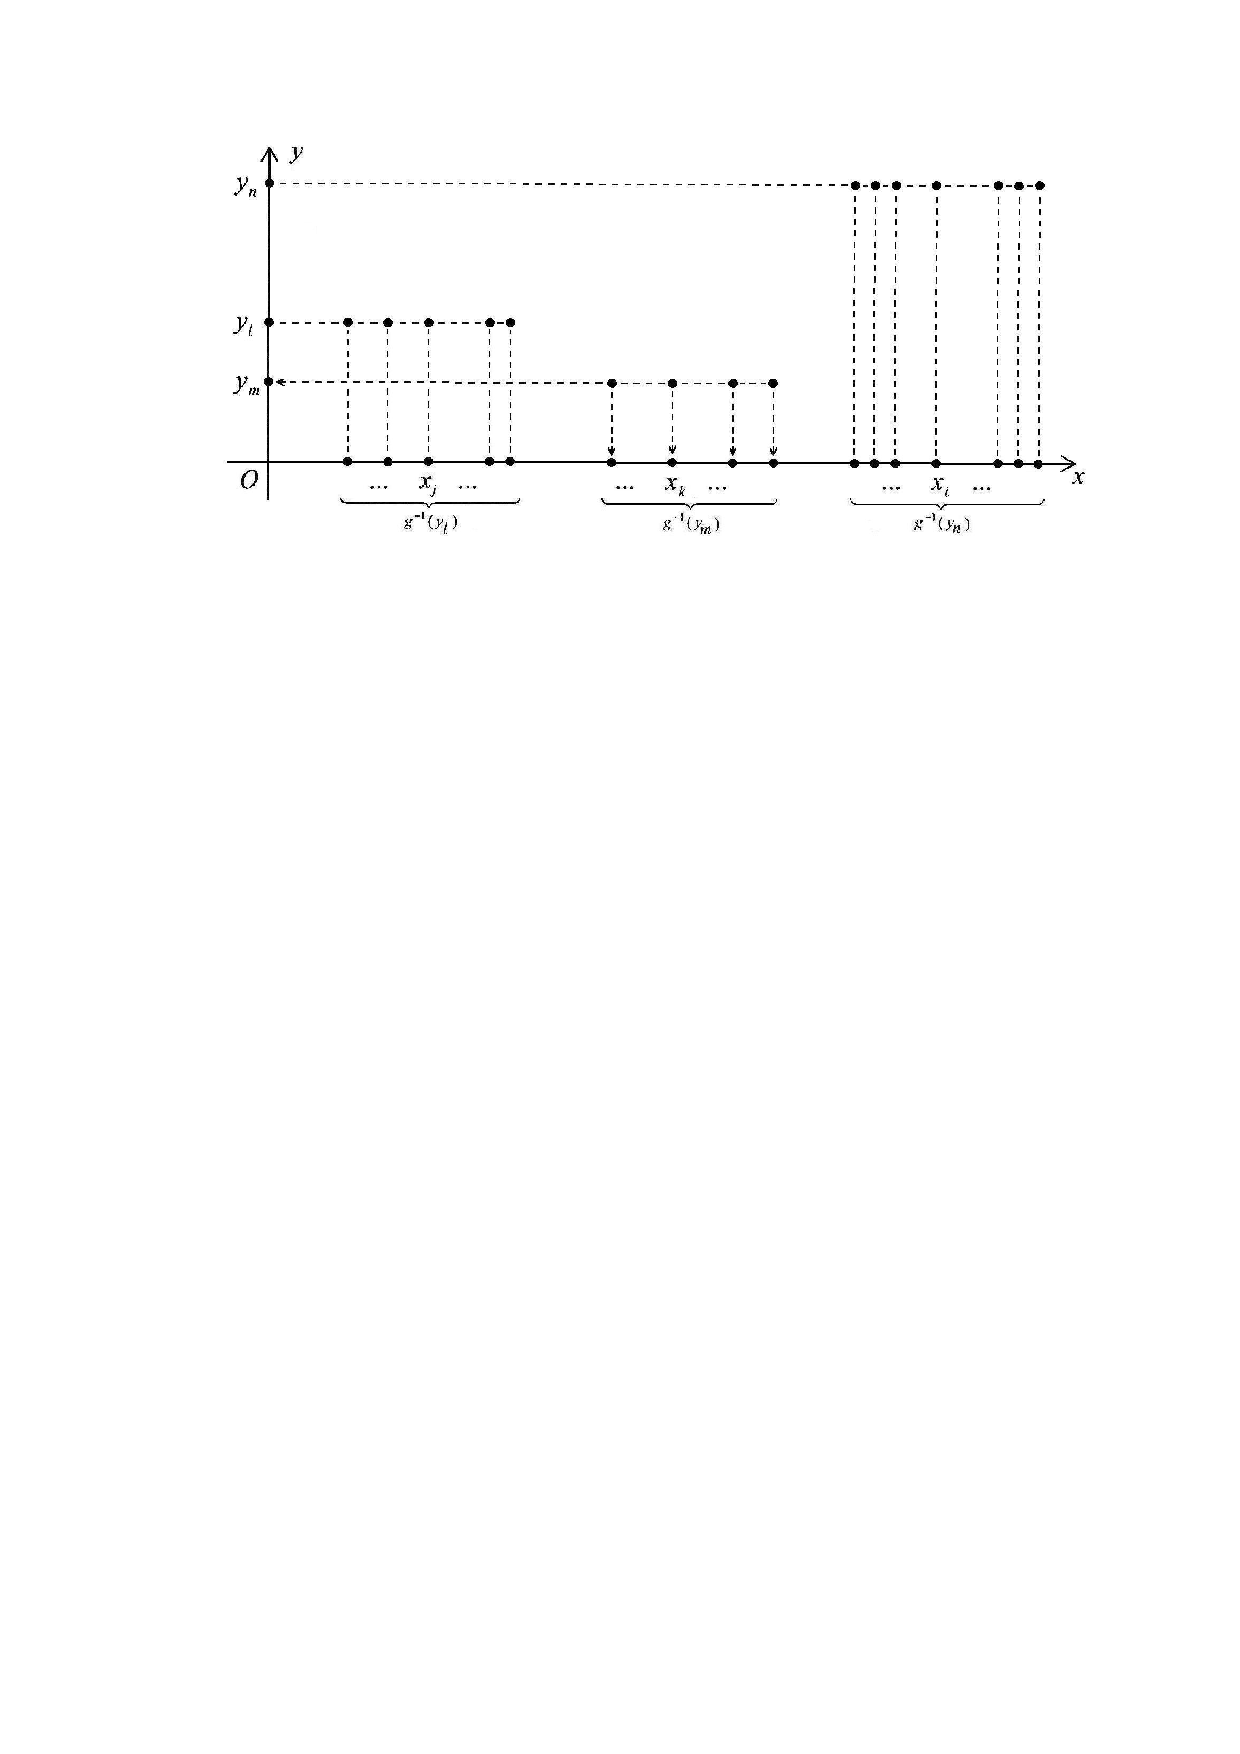
\includegraphics[]{pic/pic23}
	\caption{К доказательству теор. \ref{th:17.4}}
	\label{fig23}
\end{figure}
\begin{theorem}
\label{th:17.4}
\begin{enumerate}
	\item Для любой дискретной случайной величины $\xi$ и произвольной функции $g : \mathbb{R} \to \mathbb{R}$, математическое ожидание случайной величины $\eta = g(\xi)$ вычисляется по формуле
		\begin{equation*}
			\M\eta=\M g(\xi)=\sum_k g(x_k)p_k
		\end{equation*}
	\item Для любого абсолютно непрерывного случайного вектора
	$\xi = (\xi_1, \ldots, \xi_n) \in \mathbb{R}^n$ и произвольной функции 
	$g : \mathbb{R} \to \mathbb{R}$, математическое ожидание случайной величины 
	$\eta = g(\xi)$ вычисляется по формуле
		\begin{equation*}
			\M\eta=\M g(\xi)=\int\limits_{-\infty}^{\infty}\ldots
			\int\limits_{-\infty}^{\infty}g(t_1,\ldots,t_n)f_{\xi_1,\ldots,\xi_n}(t_1,\ldots,t_n)dt_1\ldots dt_n.
		\end{equation*}
\end{enumerate}

\end{theorem}

\begin{proof}
	Мы докажем эту теорему только для дискретного случая.
Пусть случайная величина $\xi$ принимает значения $x_1, x_2,\ldots, x_k, \ldots$ соответственно с вероятностями $p_1, p_2,\ldots , p_k,\ldots$ . Тогда $\eta= g(\xi)$ принимает
значения $y_1, y_2, \ldots , y_m, \ldots$ соответственно с вероятностями $q_1, q_2,\ldots, q_m,\ldots $, при этом полный прообраз $g^{−1}(y_m)$ может состоять из одного или более чем из одного элемента. Поэтому
	\begin{equation*}
		q_m=\P(g(\xi)=y_m)=\P(\xi\in g^{-1}(y_m))=\sum\limits
		_{x_k\in g^{-1}(y_m)}p_k.
	\end{equation*}

	Тогда
	\begin{gather*}
	\M\eta=\M g(\xi)=\sum_m y_mq_m=\sum_m y_m \sum
	\limits_{x_k\in g^{-1}(y_m)} p_k=\\=
	\sum_m\sum\limits_{x_k\in g^{-1}(y_m)}g(x_k)p_k=\sum_kg(x_k)p_k.
	\end{gather*}
	Последнее равенство справедливо потому, что суммирование по $x_k\in g^{-1}(y_m)$ означает суммирование вдоль горизонтального уровня $y = y_m$ (см. рис. \ref{fig23}), суммирование по $m$ означает суммирование сумм на горизонтальных уровнях. Поэтому двойное суммирование в левой части эквивалентно суммированию по $k$ в правой части.
\end{proof}

\begin{theorem}
Математическое ожидание имеет следующие свойства.
\begin{enumerate}
	\item Если $C = const$, то $\M C = C$.
	\item Для любой случайной величины $\xi$ имеем $\M(\M\xi) = \M\xi$.
	\item Если $C = const$, то $\M(C\xi) = C\M\xi$.
	\item Для любой случайной величины $\xi$ имеем $|\M\xi| \leqslant \M|\xi|$. 
	\item Для любых случайных величин $\xi_1$ и $\xi_2$ имеем $\M(\xi_1 + \xi_2) = \M\xi_1 +\M\xi_2.$
	\item Если случайные величины $\xi_1$ и $\xi_2$ независимы, то $\M(\xi_1\xi_2) = \M\xi_1\M\xi_2$.
\end{enumerate}
\end{theorem}

\begin{proof}
	\begin{enumerate}
		\item Константу $C$ можно рассматривать как вырожденную случайную величину $\xi = C$, сосредоточенную в точке $x = C$. Её плотность есть $f_{\xi}(x)=\delta(x-C)$. Поэтому имеем $\M\xi^n=\M C^n=\int\limits^{\infty}_{\infty} x^n\delta(x-C)dx=C^n$ и, в частности $\M C=C$

		\item Т.к. $\M\xi=const$, то $\M(\M\xi)=\M\xi$.

		\item $\M(C\xi)^n=\int\limits^{\infty}_{-\infty}(Cx)^nf_{\xi}(x)dx=C^n\int\limits^{\infty}_{-\infty}x^nf_{\xi}(x)dx=C^n\M \xi^n$
		
		\item $|\M\xi^n|=|\int\limits^{\infty}_{-\infty}x^nf_{\xi}(x)dx|\leqslant\int\limits^{\infty}_{-\infty}|x^n|f_{\xi}(x)dx=
		\M|\xi|^n$ и, в частности, $|\M\xi|\leqslant\M|\xi|$.

		\item По теор. \ref{th:17.4} и \ref{th:15.7} имеем

			\begin{gather*}
				\M(\xi_1+\xi_2)=
				\int\limits^{\infty}_{-\infty}
				\int\limits^{\infty}_{-\infty}
				(x_1+x_2)
				f_{\xi_2,\xi_2}(x_1,x_2)dx_1dx_2
				=\\=
				\int\limits^{\infty}_{-\infty}
				x_1
				\left(\int\limits^{\infty}_{-\infty} 
				f_{\xi_2,\xi_2}(x_1,x_2)dx_1dx_2
				\right)
				+
				\int\limits^{\infty}_{-\infty}
				x_2
				\left(\int\limits^{\infty}_{-\infty} 
				f_{\xi_2,\xi_2}(x_1,x_2)dx_1dx_2
				\right)
				=\\=
				\int\limits^{\infty}_{-\infty}
				x_1 f_{\xi}(x_1)dx_1+
				\int\limits^{\infty}_{-\infty}
				x_2 f_{\xi}(x_2)dx_2=
				\M\xi_1+\M\xi_2.
			\end{gather*}
		\item По теор. \ref{th:17.4}.2 и \ref{th:15.7}.4 имеем

			\begin{gather*}
				\M(\xi_1\xi_2)=
				\int\limits^{\infty}_{-\infty}\int\limits^{\infty}_{-\infty}
				x_1x_2f_{\xi_2,\xi_2}(x_1,x_2)dx_1dx_2
				=\\=
				\int\limits^{\infty}_{-\infty}
				x_1f_{\xi_2,\xi_2}(x_1,x_2)dx_1 
				\int\limits^{\infty}_{-\infty}
				x_2f_{\xi_2,\xi_2}(x_1,x_2)dx_2=
				\M\xi_2\M\xi_2
			\end{gather*}
	\end{enumerate}
\end{proof}

\begin{zam}
	Обратное утверждение, к только что доказанному свойству 6), неверно. Следующий пример показывает, что из равенства $\M(\xi_1\xi_2)=\M\xi_2\M\xi_2$ не следует независимость величин $\xi_1$ и $\xi_2$.
\end{zam}
\begin{figure}[H]
	\centering
	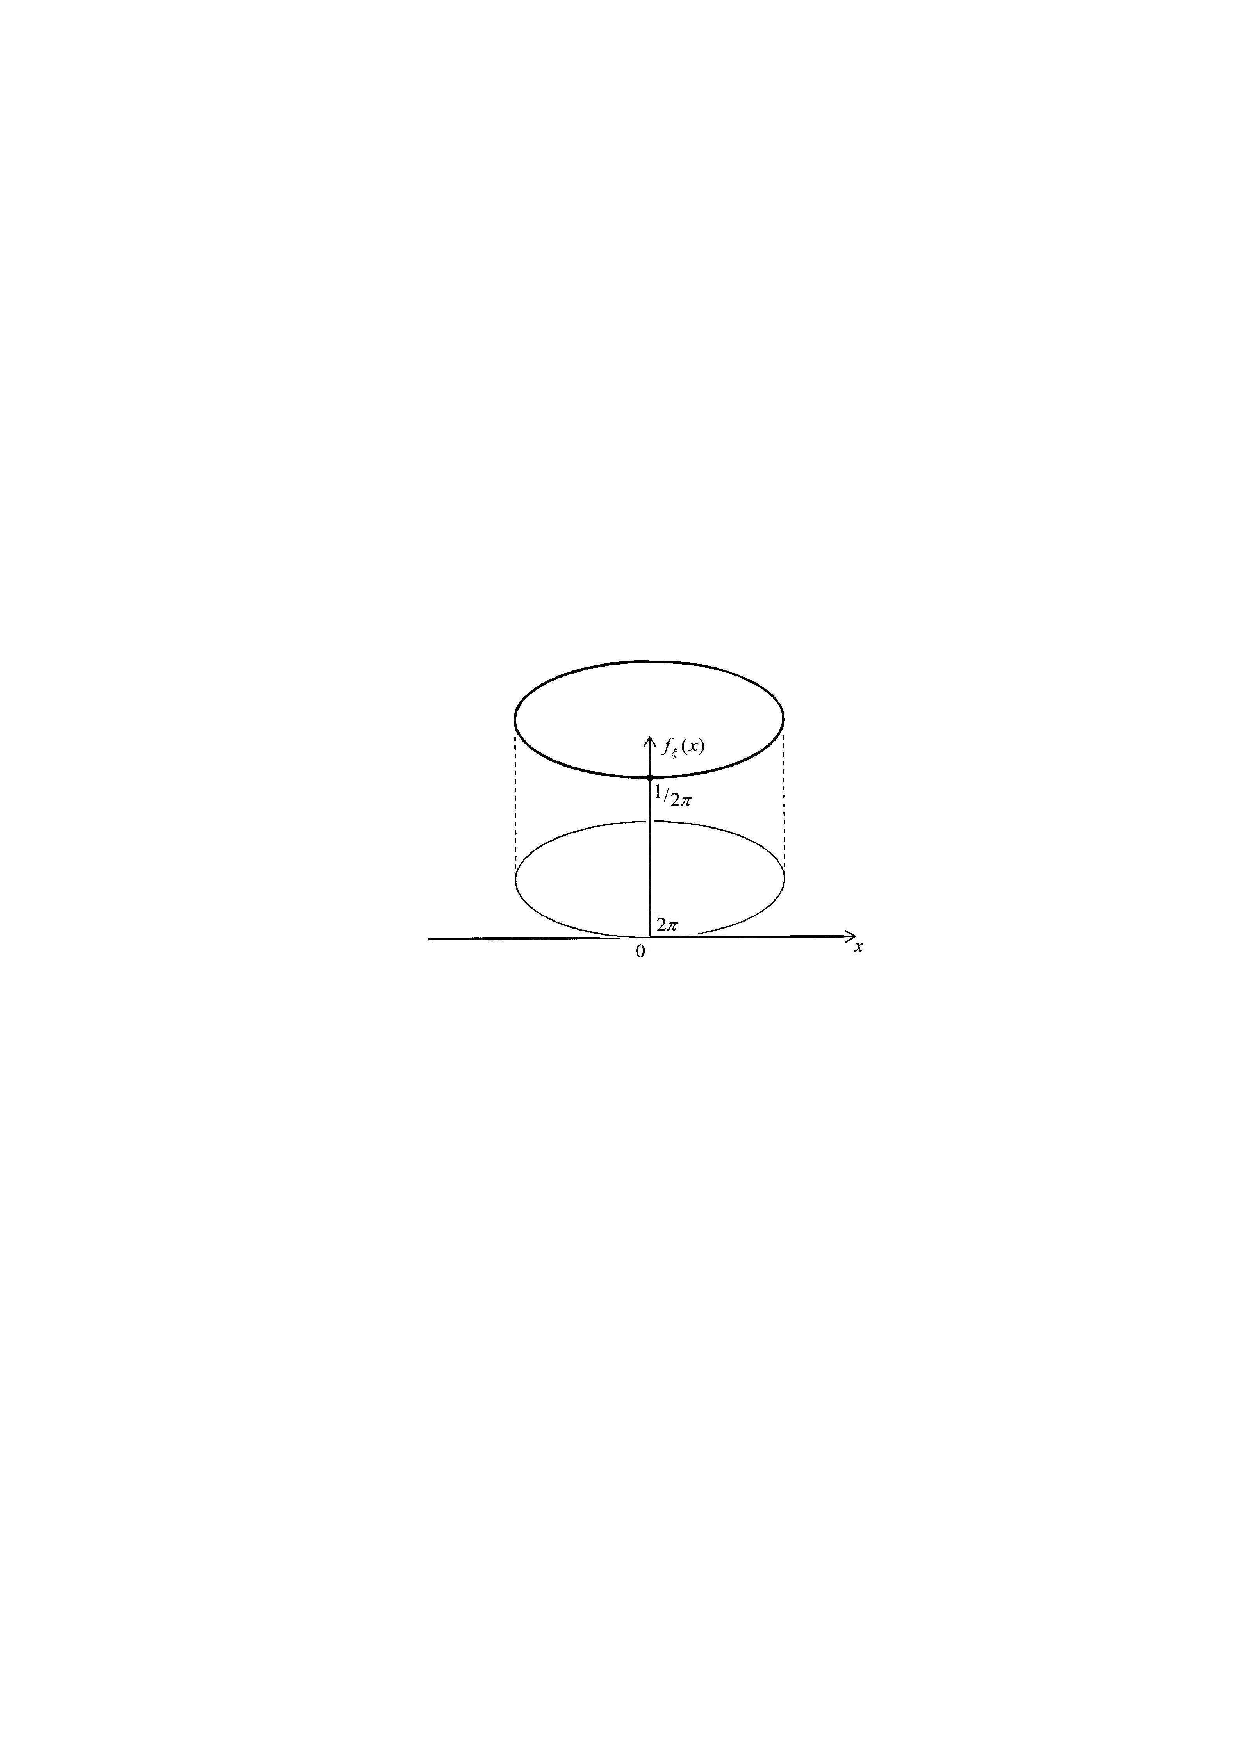
\includegraphics[]{pic/pic24}
	\caption{Равномерно распределённый угол.}
	\label{fig24}
\end{figure}

\begin{example}
	Пусть случайный угол $\phi$ равномерно распределён на окружности 
	$S^1 = \{z = e^{i\phi}\} \subset \mathbb{C} $, где $\phi\in [0, 2\pi]$. Её плотность
	\begin{equation*}
		f_{\phi}(x)=
		\begin{cases}
			\frac{1}{2\pi}, &\text{ если } x\in [0,2\pi]\\
			0, &\text{ если } x\notin [0,2\pi]\\
		\end{cases}
	\end{equation*}
	показана на рис. \ref{fig24}. Случайные величины $\xi_1 = \cos\phi$ и $\xi_2 = \sin\phi$ являются заведомо зависимыми. Ясно, что $\xi_2^2+\xi_1^2=1$. Однако математическое ожидание их произведения равно произведению их математических ожиданий.
	Действительно по теор. \ref{th:17.4} имеем

	\begin{gather*}
		\M\xi_1=\int\limits_0^{2\pi}\cos x\frac{1}{2\pi}dx=0 
		\\
		\M\xi_2=\int\limits_0^{2\pi}\sin x\frac{1}{2\pi}dx=0
		\\
		\M(\xi_1\xi_2)=\int\limits_0^{2\pi}\cos x\sin x\frac{1}{2\pi}dx=0
	\end{gather*}
\end{example}